% ex: ts=2 sw=2 sts=2 et filetype=tex
% SPDX-License-Identifier: CC-BY-SA-4.0
\begin{frame}
    \frametitle{Contenido}
    \tableofcontents
\end{frame}

\section{Introducción a Python}

\begin{frame}[c]{¿Qué es Python?}
    \begin{columns}
        \column{0.5\textwidth}
        Python es un lenguaje de programación \textit{interpretado} cuya
        filosofía hace hincapié en la \underline{legibilidad de su código}.
        Se trata de un lenguaje de programación \textbf{multiparadigma}, ya
        que soporta parcialmente la \textit{orientación a objetos,
        programación imperativa} y, en menor medida, \textit{programación
        funcional}. \\~\\

        Es un lenguaje interpretado, dinámico y multiplataforma. 
        \column{0.5\textwidth}
        \begin{center}
            
\includegraphics[scale=0.2]{python-logo.png}
        \end{center}
    \end{columns}
\end{frame}

\begin{frame}[c]{Historia}
  \begin{columns}
    \column{0.7\textwidth}
    \begin{itemize}
      \item Creado por Guido Van Rossum
      \item Holanda principios de la decade de los 90's
      \item Sintaxis simple, práctica e intuitiva
      \item De proposito general: NASA, motor de busqueda de Google, Bolsa de
        Valores de Nueva York
      \item Interpretado
      \item Multiparadigma
      \item Tipado dinámico
      \item Python 2.x ya esta \textbf{descontinuado}, solo hay que usar el 3.x
    \end{itemize}
    \column{0.3\textwidth}
        \begin{center}
            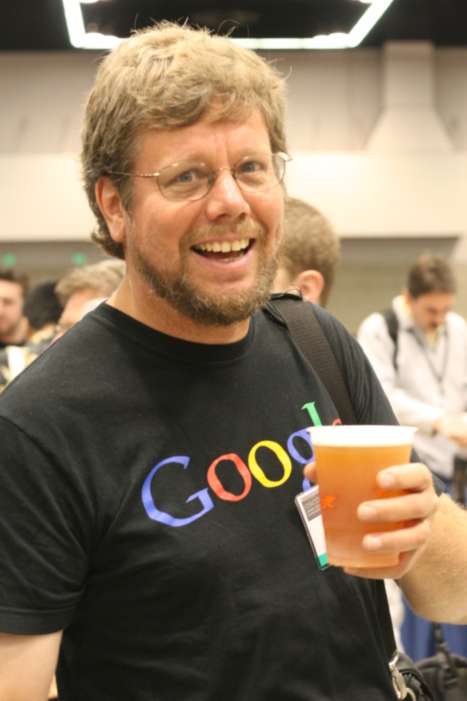
\includegraphics[scale=0.05]{Guido_van_Rossum_OSCON_2006.jpg}
        \end{center}
  \end{columns}
\end{frame}

\begin{frame}[c]{¿Qué puede hacer Python?}
  Python puede:
  \begin{itemize}
    \item ser usado en un servidor para crear aplicaciones web
    \item ser usado junto algún software para crear flojos de trajo.
    \item conectarse a un sistema de base de datos. También puede leer y
          modificar archivos.
    \item ser usado para manejar una gran cantidad de datos y funciones
          matemáticas complejas.
    \item ser usado para el desarrollo de prototipado rápido o para software
          listo para producción.
  \end{itemize}
\end{frame}

\begin{frame}[c]{Ejecución de programas}
  \begin{itemize}
    \item El código generado en Lenguaje Python se almacena en un archivo con
      extensión \textbf{.py}
  \end{itemize}
\end{frame}

\section{Reglas de codificación}

\begin{frame}[c]{Reglas de codificación}
  \begin{itemize}
    \item Los comentario de una línea inician con "\#"
    \item Los comentarios de varias líneas inician con """ y terminan con """
    \item La sangria cuenta
    \item No poner signos de putuación al final de la instrucción
    \item Es sensible a mayúsculas
    \item Errores de programación:
          \begin{itemize}
            \item Sintaxis
            \item Ejecución
            \item Lógicos
          \end{itemize}
  \end{itemize}
\end{frame}

\begin{frame}[fragile]
  \frametitle{Comentarios en Python}

  Los comentarios pueden ser usados para

  \begin{itemize}
    \item explicar el código de Python.
    \item hacer el código mas legible.
    \item prevenir la ejecución de código de pruebas.
  \end{itemize}

  \begin{lstlisting}[language=Python]
# Este es un comentario
# y otro comentario
print("Hola Mundo")

print("Hola Mundo") # Este es un comentario

# print("Hola Mundo")
print("Hello, World!")

"""
Este es un comentario
escrito en mas
de una sola linea
"""
  \end{lstlisting}
\end{frame}

\section{Variables}

\begin{frame}[fragile]
  \frametitle{Variables en Python}

  Las variables son contenedores para almacenar valores de datos.

  \begin{block}{Creando variables}
    Python no tiene un comando para declarar una variable. \\~\\
    Una variable es \textbf{creada} en el momento que se le asigna un
    valor por primera vez.
  \end{block}

  \begin{lstlisting}[language=Python]
x = 5
y = "Juan"
print(x)
print(y)
  \end{lstlisting}
\end{frame}

\begin{frame}[c]{Pantalla de inicio}
    \begin{center}
        Pantalla de inicio
    \end{center}
\end{frame}
